% !TeX spellcheck = sk_SK-Slovak
\documentclass[a4paper]{article}
\usepackage[slovak]{babel}
\usepackage[utf8]{inputenc}
\usepackage[T1]{fontenc}
\usepackage{a4wide}
\usepackage{amsmath}
\usepackage{amsfonts}
\usepackage{amssymb}
\usepackage{mathrsfs}
\usepackage[small,bf]{caption}
\usepackage{subcaption}
\usepackage{xcolor}
\usepackage{graphicx}
\usepackage{enumerate}
\usepackage{hyperref}
\usepackage{fancyvrb}
\usepackage{listings}
%\usepackage{lstautogobble}
\usepackage{stmaryrd}

\lstset{basicstyle=\ttfamily,
	mathescape=true,
	escapeinside=||%,
	%autogobble
}


\fvset{tabsize=4}


\pagestyle{empty}
\setlength{\parindent}{0pt}

\newenvironment{modenumerate}
{\enumerate\setupmodenumerate}
{\endenumerate}

\newif\ifmoditem
\newcommand{\setupmodenumerate}{%
	\global\moditemfalse
	\let\origmakelabel\makelabel
	\def\moditem##1{\global\moditemtrue\def\mesymbol{##1}\item}%
	\def\makelabel##1{%
		\origmakelabel{##1\ifmoditem\rlap{\mesymbol}\fi\enspace}%
		\global\moditemfalse}%
}

\makeatletter
\def\@seccntformat#1{%
	\expandafter\ifx\csname c@#1\endcsname\c@section\else
	\csname the#1\endcsname\quad
	\fi}
\makeatother

\begin{document} 
	
\pagenumbering{arabic}
\pagestyle{plain}

\begin{center}
	\sc\large
	Formálne metódy tvorby softvéru\\
	Domáca úloha 9
\end{center}

Autor: Marián Kravec


\section{1.)}

Po pridaní časových obmedzení vyzerá sieť ako na obrázkoch, na jednej strane toto donúti aby model neostával v jednom stave ale menil avšak tým, že neobmedzujeme počet stratení tak by stále nemalo byť zaručené, že niečo na výstupe dostaneme.
\begin{figure}[!h]
	\centering
	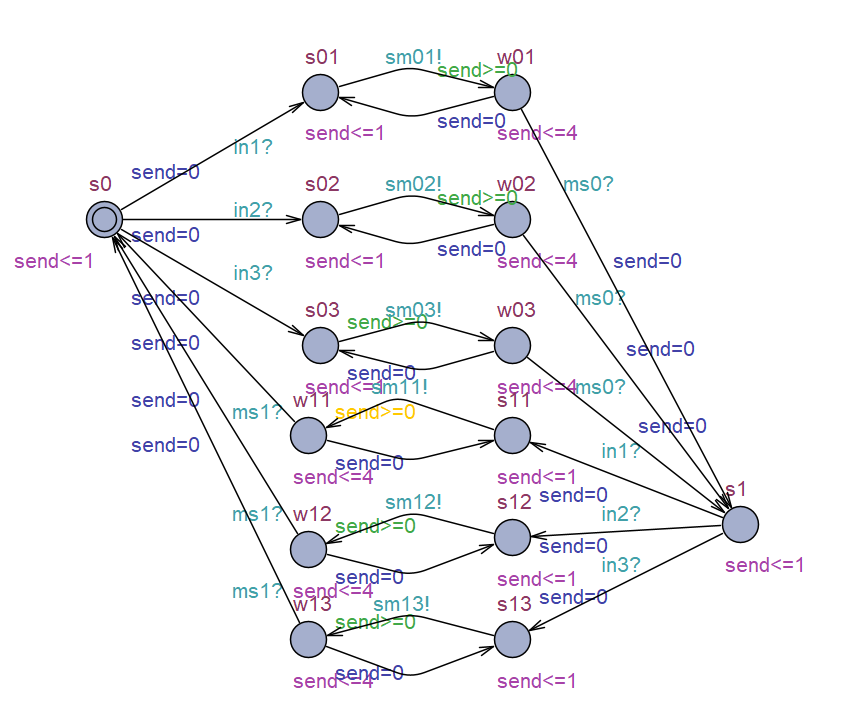
\includegraphics[width=0.7\textwidth]{s.png}
	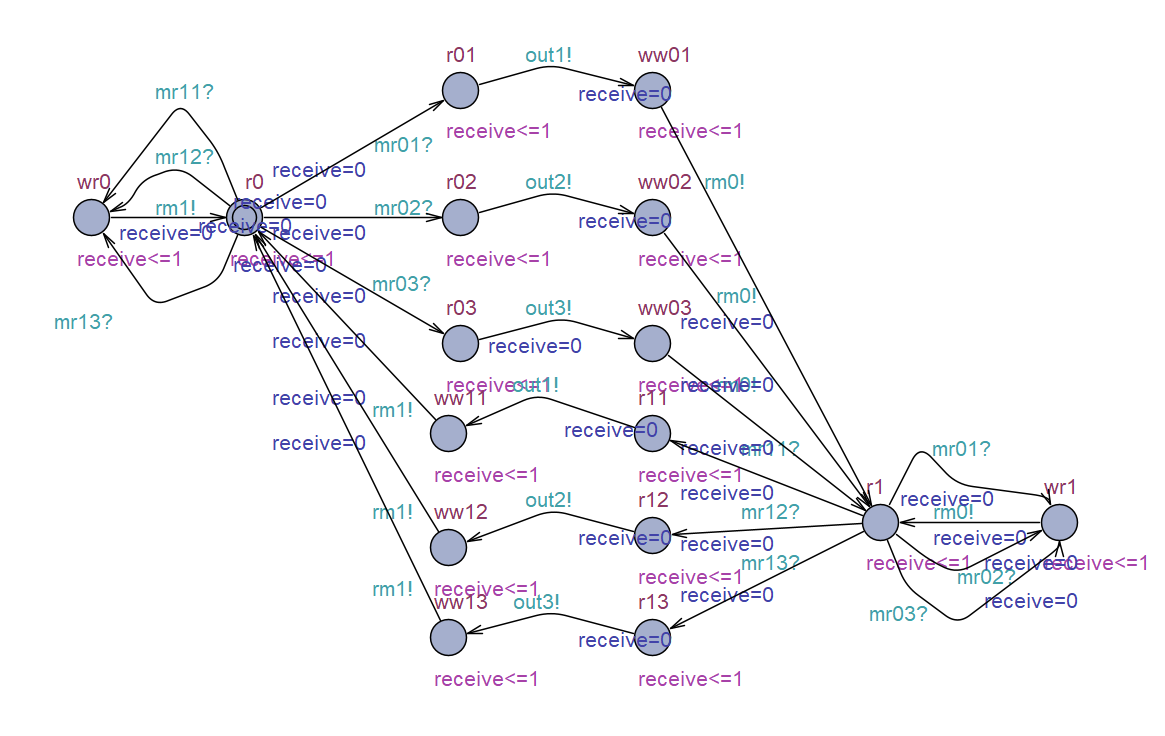
\includegraphics[width=0.7\textwidth]{r.png}
\end{figure}
\newpage

\begin{figure}[!h]
	\centering
	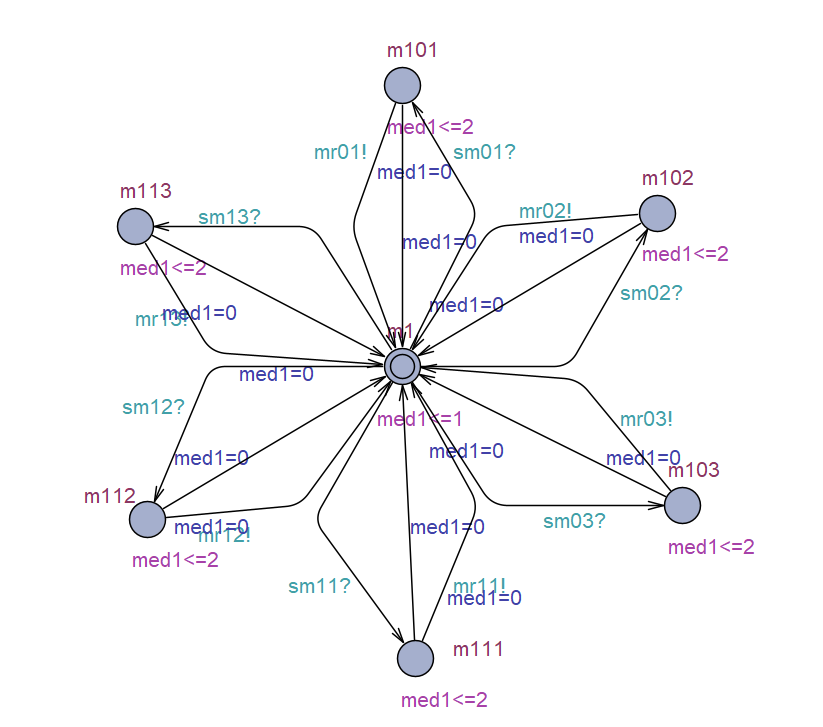
\includegraphics[width=0.7\textwidth]{m1.png}
	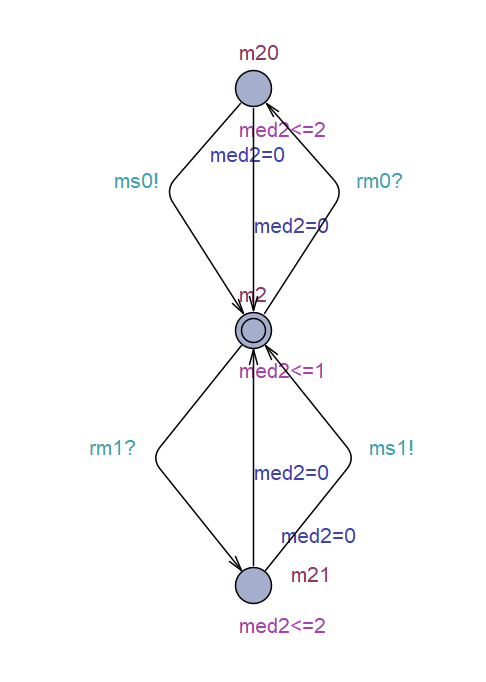
\includegraphics[width=0.5\textwidth]{m2.png}
\end{figure}
\newpage

\section{2.)}

Majme náš kód pre ABP s možnosťou stratenia jednej správy:

\begin{figure}[!h]
	\centering
	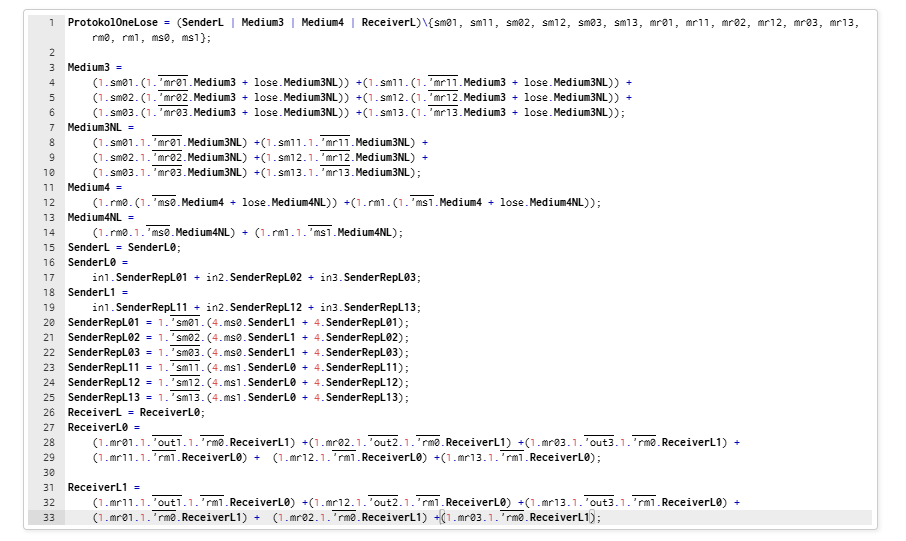
\includegraphics[width=0.7\textwidth]{ABP.png}
\end{figure}

1. ak sa správa m1 objavý na vstupe, tak sa (ako ďalšia viditeľnáakcia) raz objavý na výstupe m1.

Ja by som predpokladal, že by to malo vyzerať nejak takto, čo minimálne systém dáva, že platí.

\begin{figure}[!h]
	\centering
	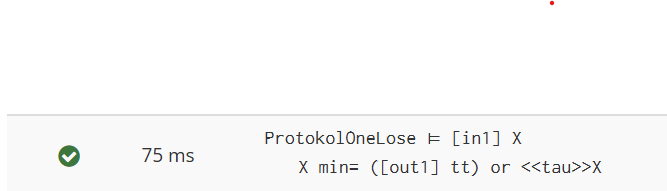
\includegraphics[width=0.7\textwidth]{1.png}
\end{figure}

2. ak neobmedzíme počet strácaní, tak toto neplatí - overte formulou.

Avšak tu nastáva problém, že aj keď obmedzím počet strát tak to stále platí... Čiže buď formula je zlá alebo som zle modifikoval kód na povolenie viac strát

\begin{figure}[!h]
	\centering
	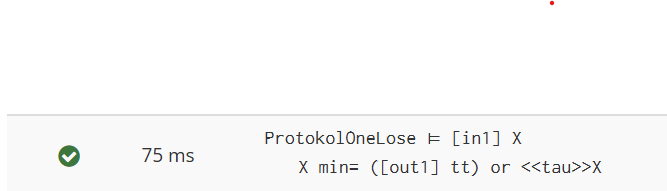
\includegraphics[width=0.7\textwidth]{1.png}
\end{figure}

3. ak sa správa m1 objavý na vstupe, tak sa ako ďalšia viditeľná akcia nemôže objaviť na výstupe správa m2.

Toto by asi malo vyzerať, nejak takto... Asi...

\begin{figure}[!h]
	\centering
	
\includegraphics[width=0.7\textwidth]{3.png}
\end{figure}
\newpage

4. pokazte Receiver tak, aby sa m2 mohlo objaviť na výstupe po m1 na vstupe a overte, 

Ach ani toto nefunguje... Myslím, že by som potreboval ešte 10 prednášok aby som pochopil tento zvrátený syntax

\begin{figure}[!h]
	\centering
	
\includegraphics[width=0.7\textwidth]{3.png}
\end{figure}

5. napíšte formulu, ktorá zaručí, v akom najhoršom čase sa správa objaví na výstupe po jej načítaní, 

Na prednáške som si začínal myslieť, že tomu čiastočne rozumiem... Absolútne nie... ABsolútne nie... 

\begin{figure}[!h]
	\centering
	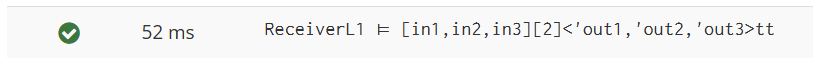
\includegraphics[width=0.7\textwidth]{5.png}
\end{figure}

6. upravte predchádzajúcu formulu (jej časové obmedznie) tak aby nebola splnená, 

Je jedno čo tam dám, ona bude splnená vždy aj keď by malo trvať minimálne 5 časových jednotiek než sa dostane z in do out... Začínam neznášať tento predmet XD.

\begin{figure}[!h]
	\centering
	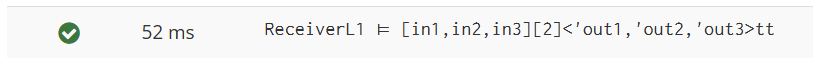
\includegraphics[width=0.7\textwidth]{5.png}
\end{figure}

7. napíšte formulu, ktorá vyjadrí po akom čase sa môže načítať ďalšia správa.

Ja už chcem mať tento predmet za sebou...

\begin{figure}[!h]
	\centering
	
\includegraphics[width=0.7\textwidth]{7.png}
\end{figure}

Skoro určite sa na to ešte pred dealinom pozriem ale zatiaľ odovzdávam toto lebo sa potrebujem sústrediť na diplomovku :P 

\end{document}